\documentclass{beamer}

\usepackage[T1]{fontenc}
\usepackage{bookman}
\usetheme[numbering=fraction, block=fill]{metropolis}  %source : https://fr.overleaf.com/latex/templates/metropolis-beamer-theme/qzyvdhrntfmr et https://mirror.foobar.to/CTAN/macros/latex/contrib/beamer-contrib/themes/metropolis/doc/metropolistheme.pdf

\usepackage{listings}
\lstset{
    showtabs=false,
    tabsize=2,
    basicstyle=\footnotesize,
    frame=single
}
\usepackage{enumitem}
\usepackage{booktabs}  % pour toprule, etc
\usepackage{amsfonts}
\usepackage{amsmath}
\usepackage{dirtree}
\usepackage{multirow}
\usepackage{amssymb}
\usepackage{cancel}
\usepackage{amsthm}
\usepackage{siunitx}
\usepackage{mathrsfs} 
\usepackage{hyperref}%   liens internet
\usepackage{tikz}
\usepackage{fourier}
\usepackage{verbatim}
\usepackage{subfigure}
\usepackage{graphicx} %Loading the package
\graphicspath{{picture/}}

\usepackage[french]{babel}

%%%%%%%%%%%%%%%%%%%%%%%%%%%%%%%%%%%%%%%%%%%%%%%%%%%%%%%%%
%Information to be included in the title page:

\title{Créer un document avec \LaTeX}
\subtitle{Rapport et autres}
\author{\href{mailto:maxime.fourquaux@heig-vd.ch}{Maxime Fourquaux}}
\institute[HEIG]%
{
    HEIG-VD -- EC+G \\
    GGT -- Géomatique et Gestion du Territoire \\
    \textbf{VERSION PROVISOIRE}
}
\date{\today}
%\logo{
\includegraphics[width=0.75cm]{HEIG-VD_logotype_rouge-rvb.eps}}
\logo{
\includegraphics[width=0.75cm]{logoEC+G_163x165_ss_txt_ssBordBlanc.png}}

%%%%%%%%%%%%%%%%%%%%%%%%%%%%%%%%%%%%%%%%%%%%%%%%%%%%%%%%%

%\newcommand*\circled[1]{\tikz[baseline=(char.base)]{
%            \node[shape=circle,draw,inner sep=2pt] (char) {#1};}}
%\newcommand{\up}[1]{\textsuperscript{#1}}
\def\labelenumi{\theenumi}
%\setbeamertemplate{enumerate item}{\alph{enumi}}
%\setbeamertemplate{enumerate subitem}{\roman{enumii}.}
%\usepackage{outline}%
%\def\labeloutlni{\theoutlni}%
%\def\theoutlni{\alph{outlni}.}%
%\renewcommand{\labelenumi}{\alph{enumi}.)

\setbeamerfont{itemize/enumerate subbody}{size=\normalsize}
\setbeamerfont{itemize/enumerate subsubbody}{size=\normalsize}
\setbeamertemplate{itemize item}{-}
\setbeamertemplate{itemize subitem}{$\checkmark$}
\setbeamertemplate{itemize subsubitem}{$\blacktriangleleft$}
%\setbeamertemplate{frame footer}{Introduction à \LaTeX -- MFX}

\newcommand{\encours}{\textit{{\color{red} En cours d'édition}}}
\newcommand{\internet}[1]{\href{#1}{{\color{red} {\footnotesize \textit{lien de téléchargement} }}}}

%\metroset{block=fill} %remplir les blocks

\makeatletter
\newcommand{\Pause}[1][]{\unless\ifmeasuring@\relax
\pause[#1]%
\fi} 
\makeatother

%%%%%%%%%%%%%%%%%%%%%%%%%%%%%%%%%%%%%%%%%%%%%%%%%%%%%%%%%
\begin{document}

{
\setbeamertemplate{frame footer}{}
\frame{\titlepage}
}

\begin{comment}
\begin{frame}{Information}
    \warning \, Ce cours est destiné à des novices. Les fonctions et autres présentées dans ce document sont celles de bases. \\
    Si vous souhaitez aller plus loin, n'hésitez à regarder la documentation sur internet et les forums !
\end{frame}
\end{comment}

\begin{frame}{Information}
    \warning Cette présentation est en cours d'écriture.
    \newline \newline 
    La version est provisoire.
    Toutes remarques, corrections, questions sont les bienvenues à (\href{mailto:maxime.fourquaux@heig-vd.ch}{Maxime Fourquaux})
\end{frame}

\section{Introduction}
\frame{
    {Historique}
    \begin{columns}
        \column{0.5\textwidth}
        \begin{itemize}
            \item Prononciation \og Lah-tec \fg{}
            \item Language et composition de document \\
                Permet de surtout se concentrer sur le fond
            \item Créé par Leslie Lamport (années 1980)
            \item Utilisé principalement dans les domaines académiques et aussi techniques
        \end{itemize}
        \column{0.5\textwidth}
        \centering
        
\includegraphics[width=0.6\textwidth]{LaTeX_logo.png}
        \\
        \vspace{1cm}
        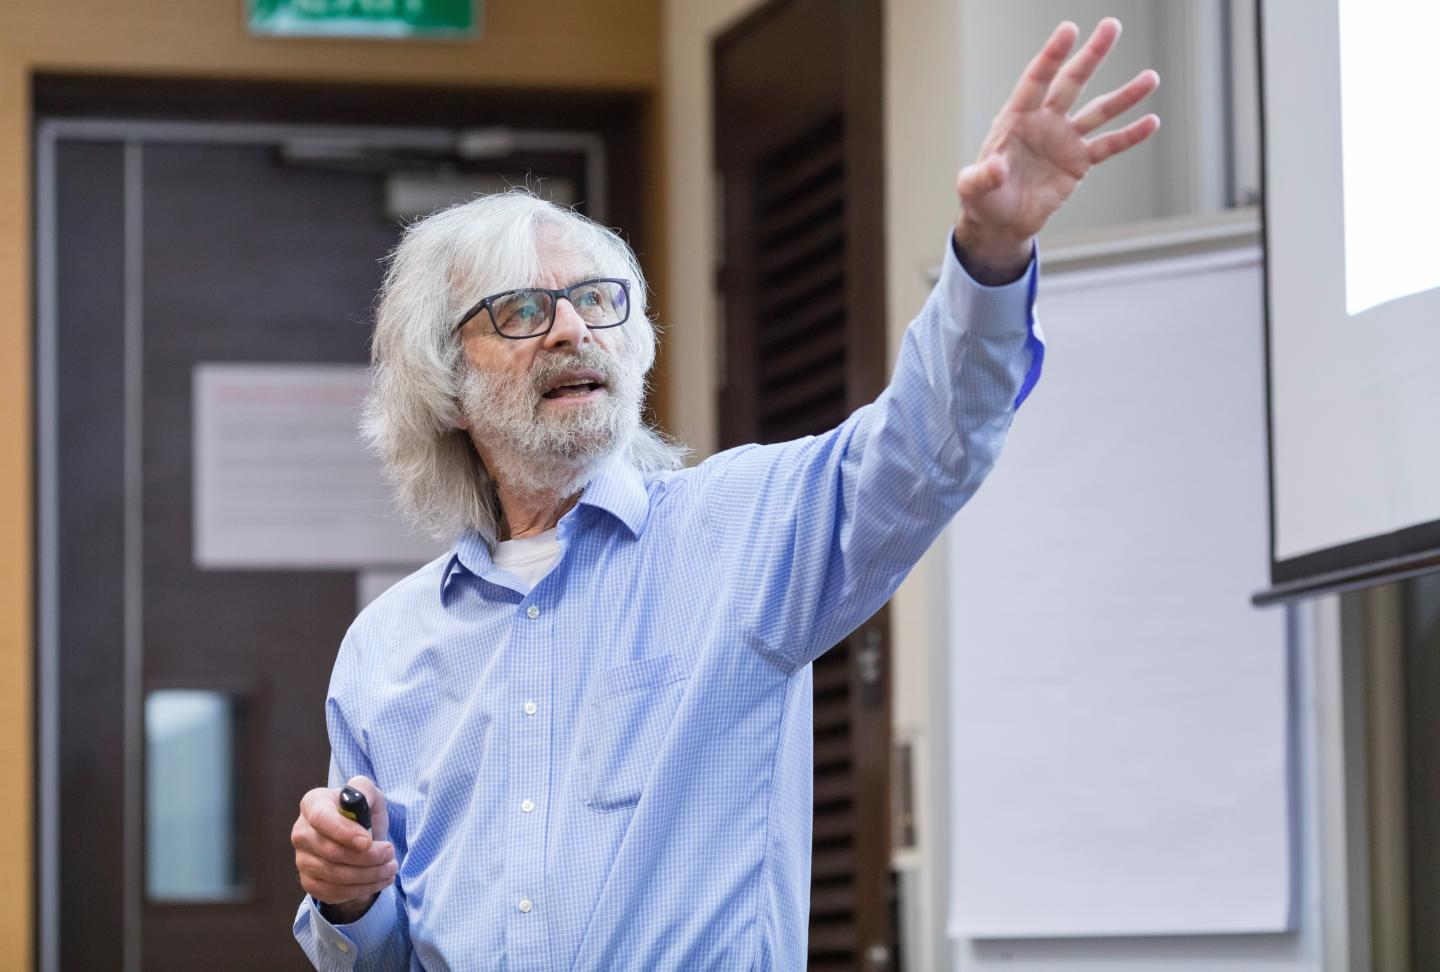
\includegraphics[width=0.6\textwidth]{Leslie_Lamport2.jpg}
    \end{columns}
}

\frame{
    {Principes d'utilisation}
    \begin{itemize}
        \item Langage informatique de balisage (comme HTML)
        \item Utiliser un éditeur de texte (NotePad++; pas MS Word)
        \item Macro-commandes et compilateur sont à utiliser
    \end{itemize}
}


\begin{frame}{Table des matières}
  \setbeamertemplate{section in toc}[sections numbered]
  \tableofcontents%[hideallsubsections]
\end{frame}

\section{Créer son premier document \LaTeX}

\begin{frame}[containsverbatim]
    \frametitle{Généralités}
    \encours
    \begin{comment}
        Extension de fichier
        Compilation
        Ecriture
        balises, ...
    \end{comment}
\end{frame}

\begin{frame}[containsverbatim]
    \frametitle{Bases du document \LaTeX}
    \begin{lstlisting}[language=TeX, caption=Contenu minimal d'un document \texttt{.tex}]
        \documentclass[11pt]{book}
        \usepackage[T1]{fontenc}
        \begin{document}
            Bonjour
        \end{document}
    \end{lstlisting}
\end{frame}


\section{Structure (paragraphes, \dots)}

\begin{frame}[containsverbatim]
    \frametitle{Chapitres, paragraphes, \dots}
    \begin{table}
        \centering
        \begin{tabular}{|l|l|}
            \hline
            Partie            & \verb|\part{titre}| \\
            \hline
            Chapitre          & \verb|\chapter{titre}| \\
            \hline
            Section           & \verb|\section{titre}| \\
            \hline
            Sous-section      & \verb|\subsection{titre}| \\
            \hline
            Sous-sous-section & \verb|\subsubsection{titre}| \\
            \hline
            Paragraphe        & \verb|\paragraph{titre}| \\
            \hline
        \end{tabular}
    \end{table}
    
\end{frame}

\begin{frame}{Exemples -- Chapitres, paragraphes, \dots}
    \encours
\end{frame}

\begin{frame}[containsverbatim]
    \frametitle{Absence de numérotation}
    Il est parfois utile de ne pas numéroter un chapitre ou une section (par exemple l'introduction).
    Il suffit pour cela d'ajouter un astérix (*) après le chapitre. \\
    Exemple : \verb|\chapter*{titre}|
    \bigskip
    \begin{exampleblock}{Ajouter le titre non numéroté au sommaire}
        \encours
    \end{exampleblock}
\end{frame}
\section{Mise en forme du texte}

\begin{frame}[containsverbatim]
    \frametitle{Mise en forme du texte}
    \begin{table}
        \centering
        \begin{tabular}{|c||c|c|}
            \hline
            Gras     & \textbf{géodésie}    & \verb|\textbf{géodésie}| \\
            \hline
            Italique & \textit{géodésie}    & \verb|\textit{géodésie}| \\
            \hline
            Souligné & \underline{géodésie} & \verb|\underline{géodésie}| \\
            \hline
            Télétype & \texttt{géodésie} & \verb|\texttt{géodésie}| \\
            \hline
            Sans-sérif & \textsf{géodésie} & \verb|\textsf{géodésie}| \\
            \hline
            Incliné & \textsl{géodésie} & \verb|\textsl{géodésie}| \\
            \hline
            Petites majuscules & \textsc{géodésie} & \verb|\textsc{géodésie}| \\
            \hline
        \end{tabular}
    \end{table}
\end{frame}

\begin{frame}[containsverbatim]
    \frametitle{Taille de police}
    \begin{table}
        \centering
        \begin{tabular}{|c|c|}
            \hline
            \tiny{géodésie} & \verb|\tiny{géodésie}| \\
            \hline
            \scriptsize{géodésie} & \verb|\scriptsize{géodésie}| \\
            \hline
            \footnotesize{géodésie} & \verb|\footnotesize{géodésie}| \\
            \hline
            \small{géodésie} & \verb|\small{géodésie}| \\
            \hline
            \normalsize{géodésie} & \verb|\normalsize{géodésie}| \\
            \hline
            \large{géodésie} & \verb|\large{géodésie}| \\
            \hline
            \Large{géodésie} & \verb|\Large{géodésie}| \\
            \hline
            \LARGE{géodésie} & \verb|\LARGE{géodésie}| \\
            \hline
            \huge{géodésie} & \verb|\huge{géodésie}| \\
            \hline
            \Huge{géodésie} & \verb|\Huge{géodésie}| \\
            \hline
        \end{tabular}
    \end{table}
\end{frame}

\begin{frame}[containsverbatim]
    \frametitle{Modification de la taille de la police}
    \begin{lstlisting}[language=TeX, caption=Différentes manières]
    a {\Large texte} b
    a \Large texte \normalsize b
    a \begin{Large}texte\end{Large} b
    \end{lstlisting}
    \begin{exampleblock}{Résultat}
        a {\Large géodésie} b
    \end{exampleblock}
    \begin{alertblock}{Attention}
        Ce sont des tailles relatives par rapport à la taille de police définie dans la première ligne du \texttt{main.tex}
    \end{alertblock}
\end{frame}
\section{Écrire des mathématiques}

\begin{frame}{Packages minimum utiles}
    \begin{itemize}[label=$\triangleright$]
        \item \texttt{amsfonts}
        \item \texttt{amsmath}
        \item \texttt{amssymb}
        \item \texttt{amsthm}
    \end{itemize}
\end{frame}

\begin{frame}[containsverbatim]
    \frametitle{Environnements différents}
    \begin{exampleblock}{En ligne}
        Savez-vous que $\pi=3.14$ ?
    \end{exampleblock}
    \begin{lstlisting}[language=TeX]
        Savez-vous que $\pi=3.14$ ?
    \end{lstlisting}
    \bigskip
    \begin{exampleblock}{Hors-ligne}
        Savez-vous que \[ \pi=3.14 \] ?
    \end{exampleblock}
    \begin{lstlisting}[language=TeX]
        Savez-vous que \[ \pi=3.14 \] ?
    \end{lstlisting}
\end{frame}

\begin{frame}[containsverbatim]
    \frametitle{Équations hors-ligne}
    \begin{exampleblock}{Numérotée}
        L'équation de l'Univers est :
        \begin{equation}
            e = m\cdot c^2
        \end{equation}
    \end{exampleblock}
    \begin{lstlisting}[language=TeX]
        L'equation de l'Univers est :
        \begin{equation}
            e = m \cdot c^2
        \end{equation}
    \end{lstlisting}
    \bigskip
\end{frame}

\begin{frame}[containsverbatim]
    \frametitle{Équations hors-ligne}
    \begin{exampleblock}{Non numérotée}
        L'équation de l'Univers est :
        \begin{equation*}
            e = m\cdot c^2
        \end{equation*}
    \end{exampleblock}
    \begin{lstlisting}[language=TeX]
    L'equation de l'Univers est :
    \begin{equation*}
    e = m \cdot c^2
    \end{equation*}
    \end{lstlisting}
    \bigskip
\end{frame}

\begin{frame}[containsverbatim]
    \frametitle{Exemples d'équations}
    \begin{columns}
        \column{0.3\textwidth}
        \begin{align*}
            m &= \cfrac{e}{c^{2}} \\
            c &= \pm \sqrt{\cfrac{e}{m}}
        \end{align*}
        \begin{equation*}
            \sin^2 x + \cos^2 x = 1
        \end{equation*}
        \begin{align*}
            \displaystyle{\int_3^{6x} x^3 + \sin^2 dx} \\ 
            \displaystyle{\mathbf{\mu_{Y}} \approx \mathbf{f(x)} + \cfrac{\partial \mathbf{f}}{\partial \mathbf{x}} \cdot \Delta \mathbf{x}}
        \end{align*}
        \column{0.7\textwidth}
        \footnotesize
        \begin{lstlisting}[language=TeX]
        \begin{align*}
        m &= \cfrac{e}{c^{2}} \\
        c &= \pm \sqrt{ \cfrac{e}{m} }
        \end{align*}
        \end{lstlisting}
        \begin{lstlisting}[language=TeX]
        \begin{equation*}
        \sin^2 x + \cos^2 x = 1
        \end{equation*}
        \end{lstlisting}
        \begin{lstlisting}[language=TeX]
        \begin{align*}
        \int_3^{6x} x^3 + \sin^2 dx \\ 
        \mathbf{\mu_{Y}} \approx 
        \mathbf{f(x)} + 
        \cfrac{\partial \mathbf{f}}
        {\partial \mathbf{x}} \cdot 
        \Delta \mathbf{x}
        \end{align*}
        \end{lstlisting}
    \end{columns}
\end{frame}

\begin{frame}[containsverbatim]
    \frametitle{Différentes matrices}
    \footnotesize
    \begin{table}
        \centering
        \begin{tabular}{ll}
            \verb|{matrix}|  & : matrice sans délimitateur    \\
            \verb|{pmatrix}| & : matrice entre parenthèses    \\
            \verb|{vmatrix}| & : matrice entre barres         \\
            \verb|{Vmatrix}| & : matrice entre doubles barres \\
            \verb|{bmatrix}| & : matrice entre croches        \\
            \verb|{Bmatrix}| & : matrice entre accolades      \\
        \end{tabular}
    \end{table}
    \begin{columns}
        \column{0.3\textwidth}
        \begin{center}
            $\begin{matrix} a&b \\ c&d \end{matrix} \qquad \begin{pmatrix} a&b \\ c&d \end{pmatrix}$
            $\begin{vmatrix} a&b \\ c&d \end{vmatrix} \qquad \begin{Vmatrix} a&b \\ c&d \end{Vmatrix}$
            $\begin{bmatrix} a&b \\ c&d \end{bmatrix} \qquad \begin{Bmatrix} a&b \\ c&d \end{Bmatrix}$
        \end{center}
        \column{0.7\textwidth}
        \verb|$\begin{matrix} a&b\\ c&d \end{matrix}$|   \\
        \verb|$\begin{pmatrix} a&b\\ c&d \end{pmatrix}$| \\
        \verb|$\begin{vmatrix} a&b\\ c&d \end{vmatrix}$| \\
        \verb|$\begin{Vmatrix} a&b\\ c&d \end{Vmatrix}$| \\
        \verb|$\begin{bmatrix} a&b\\ c&d \end{bmatrix}$| \\
        \verb|$\begin{Bmatrix} a&b\\ c&d \end{Bmatrix}$| \\
    \end{columns}
\end{frame}

\begin{frame}[containsverbatim]
    \frametitle{Divers symboles et polices}
    \begin{table}
        \centering
        \begin{tabular}{|c|l|l|}
            \hline
            $\mathrm{x=\sqrt{2}}$ & \verb|\mathrm{...}|     & romaine    \\ 
            \hline
            $\mathit{x=\sqrt{2}}$ & \verb|\mathit{...}|     & italique   \\
            \hline
            $\mathtt{x=\sqrt{2}}$ & \verb|\mathtt{...}|     & télétype   \\ 
            \hline
            $\mathbf{x=\sqrt{2}}$ & \verb|\mathbf{...}|     & gras       \\
            \hline
            $\mathsf{x=\sqrt{2}}$ & \verb|\mathsf{...}|     & sans-serif \\
            \hline
            $\mathbb{ABC}$        & \verb|\mathbb{ABC}|     & \\
            \hline
            $\mathcal{ABC}$       & \verb|\mathcal{ABC}|    & \\
            \hline
            $\mathscr{ABC}$       & \verb|\mathscr{ABC}|    & \\
            \hline
            $\mathfrak{ABC}$      & \verb|\mathfrak{ABC}|   & \\
            \hline
            $\mathnormal{ABC}$    & \verb|\mathnormal{ABC}| & \\
            \hline
        \end{tabular}
    \end{table}
\end{frame}

\begin{frame}[containsverbatim]
    \frametitle{Divers symboles et polices}
    \begin{table}
        \centering
        \begin{tabular}{|c|l|}
            \hline
            $\vec{x}$             & \verb|\vec{x}|             \\
            \hline
            $\overrightarrow{AB}$ & \verb|\overrightarrow{AB}| \\
            \hline
            $\cancel{x}$          & \verb|\cancel{x}|          \\
            \hline
            $\bcancel{x}$         & \verb|\bcancel{x}|         \\
            \hline
            $\xcancel{x}$         & \verb|\xcancel{x}|         \\
            \hline
        \end{tabular}
    \end{table}
    \begin{figure}
        \centering
        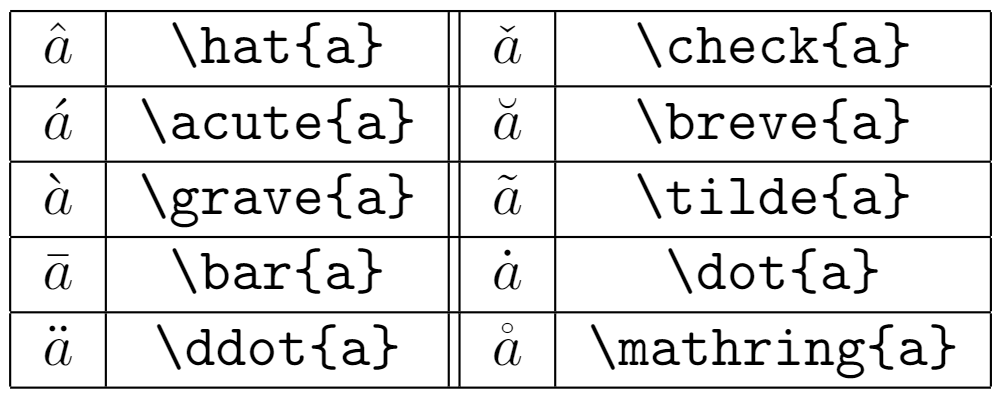
\includegraphics[width=7cm]{accentMathematiques.png}
    \end{figure}
\end{frame}

\begin{frame}[containsverbatim]
    \frametitle{Lettres grecques}
    \begin{table}
        \centering
        \begin{tabular}{|c|l||c|l||c|l|}
            \hline
            $\alpha$    & \verb|\alpha|    & $\beta$    & \verb|\beta|    & $\gamma$      & \verb|\gamma|      \\
            $\delta$    & \verb|\delta|    & $\epsilon$ & \verb|\epsilon| & $\varepsilon$ & \verb|\varepsilon| \\
            $\zeta$     & \verb|\zeta|     & $\eta$     & \verb|\eta|     & $\theta$      & \verb|\theta|      \\
            $\vartheta$ & \verb|\vartheta| & $\iota$    & \verb|\iota|    & $\kappa$      & \verb|\kappa|      \\
            $\lambda$   & \verb|\lambda|   & $\mu$      & \verb|\mu|      & $\nu$         & \verb|\nu|         \\
            $\xi$       & \verb|\xi|       & $\pi$      & \verb|\pi|      & $\varpi$      & \verb|\varpi|      \\
            $\rho$      & \verb|\rho|      & $\varrho$  & \verb|\varrho|  & $\sigma$      & \verb|\sigma|      \\
            $\varsigma$ & \verb|\varsigma| & $\tau$     & \verb|\tau|     & $\upsilon$    & \verb|\upsilon|    \\
            $\phi$      & \verb|\phi|      & $\varphi$  & \verb|\varphi|  & $\chi$        & \verb|\chi|        \\
            $\psi$      & \verb|\psi|      & $\omega$   & \verb|\omega|   &               &                    \\
            \hline
        \end{tabular}
    \end{table}
\end{frame}

\begin{frame}[containsverbatim]
    \frametitle{Lettres grecques}
    \begin{table}
        \centering
        \begin{tabular}{|c|l||c|l|}
            \hline
            $\Gamma$ & \verb|\Gamma| & $\Delta$   & \verb|\Delta|   \\
            $\Theta$ & \verb|\Theta| & $\Lambda$  & \verb|\Lambda|  \\
            $\Xi$    & \verb|\Xi|    & $\Pi$      & \verb|\Pi|      \\
            $\Sigma$ & \verb|\Sigma| & $\Upsilon$ & \verb|\Upsilon| \\
            $\Phi$   & \verb|\Phi|   & $\Psi$     & \verb|\Psi|     \\
            $\Omega$ & \verb|\Omega| &            &                 \\
            \hline
        \end{tabular}
    \end{table}
\end{frame}
\section{Références et tables}

\begin{frame}[containsverbatim]
    \frametitle{Création de référence}
    \begin{alertblock}{Explication}
        Il est tout à possible de créer une \og ancre \fg{} à un paragraphe, une équation ou une figure ou tout autre élément de votre choix. \\
        La commande à utiliser est : \verb|\label{}|
    \end{alertblock}
    \begin{lstlisting}[language=TeX, caption=Exemple]
    \begin{equation}\label{eq:relativite}
        e = m \cdot c^2
    \end{equation}
    \end{lstlisting}
    \begin{equation}\label{eq:relativite}
        e = m \cdot c^2
    \end{equation}
\end{frame}

\begin{frame}[containsverbatim]
    \frametitle{Référence à une ancre}
    \begin{alertblock}{Explication}
        Faire référence à une ancre est une méthode générique. \\
        Pour cela, la commande à utiliser est : \verb|\ref{}|.
    \end{alertblock}
    \begin{lstlisting}[language=TeX, caption=Exemple]
    L'equation \ref{eq:relativite} est la formule de la
    relavitive generale.
    \end{lstlisting}
    L'équation \ref{eq:relativite} est la formule de la relativité générale.
\end{frame}

\begin{frame}[containsverbatim]
    \frametitle{Référence à une page}
    \begin{alertblock}{Explication}
        On veut parfois savoir à quelle page se situe l'objet dont on fait la référence. \\
        Pour cela, on peut utiliser la commande : \verb|\pageref{}|
    \end{alertblock}
    \begin{lstlisting}[language=TeX, caption=Exemple]
    L'equation \ref{eq:relativite}, page
    \pageref{eq:relativite} est la formule de la 
    relavitive generale.
    \end{lstlisting}
    L'équation \ref{eq:relativite}, page \pageref{eq:relativite} est la formule de la relativité générale.
    \end{frame}

\begin{frame}[containsverbatim]
    \frametitle{Référence à l'objet courant}
    \begin{alertblock}{Explication}
        Il est courant de faire référence parfois au chapitre, ou section dans lequel on se trouve. \\
        Pour cela on utilise des commandes : \texttt{the}-commandes.
    \end{alertblock}
    \begin{lstlisting}[language=TeX, caption=Exemple]
    Nous sommes actuellement dans la section \thesection.
    \end{lstlisting}
    Nous sommes actuellement dans la section \thesection.
\end{frame}

\begin{frame}[containsverbatim]
    \frametitle{Création d'une table (ou liste)}
    \begin{alertblock}{Explication}
        Grâce à la structure du document (chapitres, images, tableaux, \dots), il est possible d'obtenir la table des matières et les tables d'images aisément. \\
        De plus, en compilant le fichier, les tables se mettent à jour automatiquement ; ainsi que les références etc.
    \end{alertblock}
    \footnotesize
    \begin{table}
        \centering
        \begin{tabular}{|l|l|}
            \hline
            \verb|\tableofcontents| & Table des matières  \\
            \verb|\listoffigures|   & Liste des figures   \\
            \verb|\listoftables|    & Listes des tableaux \\
            \hline
        \end{tabular}
    \end{table}
    \begin{exampleblock}{Nota}
        Il n'est pas possible de créer une table des équations comme on fait pour les images. \\
        Il existe d'autres alternatives en créant une macro qui légende les équations ou alors de créer un index avec des mots particuliers.
    \end{exampleblock}
\end{frame}
\normalsize

\section{Figures, importation et création}

\begin{frame}{Notes}
    \begin{alertblock}{Package}
        Pour importer des images dans votre document, il faut utiliser le package \texttt{graphicx}.
        Sans lui vous pourrez importer des images dans le document \texttt{.tex} mais elles n'apparaîtront pas dans le \texttt{.pdf}.
    \end{alertblock}
\end{frame}

\begin{frame}[containsverbatim]
    \frametitle{Importation d'une figure}
    \begin{exampleblock}{Contenu minimal recommandé}
        \begin{figure}
            \centering
            
\includegraphics[scale=0.2]{LaTeX_logo.png}
            \caption{Logo de \LaTeX}
            \label{fig:logoLatex}
        \end{figure}
    \end{exampleblock}
    \begin{lstlisting}[language=TeX]
        \begin{figure}
            \centering
            
\includegraphics[scale=0.2]{LaTeX_logo.png}
            \caption{Logo de \LaTeX} %la table des figs.
            \label{fig:logoLatex} %utile pour les cf.
        \end{figure}
    \end{lstlisting}
\end{frame}

\begin{frame}[containsverbatim]
    \frametitle{Divers paramètres}
    \begin{exampleblock}{Contenu minimal recommandé}
        \begin{figure}
            \centering
            
\includegraphics[width=1cm, angle=35]{LaTeX_logo.png}
            \caption{Logo de \LaTeX}
        \end{figure}
    \end{exampleblock}
    \begin{lstlisting}[language=TeX]
        \begin{figure}
            \centering
            
\includegraphics[width=1cm, angle=160]{LaTeX_logo.png}
            \caption{Logo de \LaTeX}
            \label{fig:logoLatex}
        \end{figure}
    \end{lstlisting}
\end{frame}


\begin{frame}[containsverbatim]
    \frametitle{Dessin vectoriel}
    \begin{alertblock}{Packages possibles}
        \begin{itemize}[label=$\triangleright$]
            \item \texttt{tikz}
            \item \texttt{pstricks}
            \item \texttt{pst-node}
        \end{itemize}
    \end{alertblock}
    \begin{alertblock}{Alternatives}
        Importer directement des fichiers vectoriels avec les extensions adéquats (\texttt{*.eps}, \texttt{*.svg}, \dots) \\
        ou bien \\
        Le site internet \href{https://www.mathcha.io/}{https://www.mathcha.io/} qui permet de créer le dessin et générer le code TeX
    \end{alertblock}
\end{frame}
\section{Créer des tableaux}

\begin{frame}[containsverbatim]
    \frametitle{Créer un tableau}
    \begin{table}
        \centering
        \begin{tabular}{|r||l|l|c|}
            \hline
            \textbf{ID} & \textbf{E. RGF93} & \textbf{N. RGF93} & \textbf{Alt.} \\
            \hline \hline
            I.AB - 54      & 967.03 & 6591.37  & 436.573    \\
            \hline
            I.A.K3 - 51bis & 967.47 & 6591.42  & 431.091    \\
            \hline
        \end{tabular}
    \end{table}
    \begin{lstlisting}[language=TeX]
    \begin{table}
        \centering
        \begin{tabular}{|r||l|l|c|}
            \hline
            ID & E. RGF93 & N. RGF93 & Alt. \\
            \hline \hline
            I.AB - 54 & 967.03 & 6591.37 & 436.573 \\
            \hline
        \end{tabular}
    \end{table}
    \end{lstlisting}
\end{frame}

\begin{frame}[containsverbatim]
    \frametitle{Cellules multicolonnes}
    \begin{table}
        \centering
        \begin{tabular}{c|c|c|c}
            \multicolumn{2}{c|}{\textbf{CH1903+}} & \multicolumn{2}{|c}{\textbf{WGS84}} \\
            \hline
            2500875.98 & 1117944.47 & \ang{46,20564} & \ang{6,15430} \\
            2540407.43 & 1181157.61 & \ang{46,77892} & \ang{6,65830} \\
            \hline
        \end{tabular}
    \end{table}
    \footnotesize
    \begin{lstlisting}[language=TeX]
    \begin{table}
        \centering
        \begin{tabular}{c|c|c|c}
            \multicolumn{2}{|c|}{\textbf{CH1903+}} & 
            \multicolumn{2}{|c}{\textbf{WGS84}} \\
            \hline
            2500875.98 & 1117944.47 & 46,20564 & 6,15430 \\
            2540407.43 & 1181157.61 & 46,77892 & 6,65830 \\
            \hline
        \end{tabular}
    \end{table}
    \end{lstlisting}
\end{frame}


\begin{frame}[containsverbatim]
    \frametitle{Cellules multilignes}
    \begin{table}
        \centering
        \begin{tabular}{|c|c|}
            \hline
            \multirow{2}{*}{Admis} & Non redoublants \\
            \cline{2-2}
                                   & Redoublants     \\
            \hline
        \end{tabular}
    \end{table}
    \begin{lstlisting}[language=TeX]
    \begin{tabular}{|c|c|}
        \hline
        \multirow{2}{*}{Admis} & Non redoublants \\
        \cline{2-2}
                               & Redoublants     \\
        \hline
    \end{tabular}
    \end{lstlisting}
\end{frame}


\begin{frame}[containsverbatim]
    \frametitle{Mémo}
    \begin{itemize}[label=$\triangleright$]
        \item Cellule multicolonne : \verb|\multicolumn{nombre}{col}{texte}|
        \item Cellule multiligne : \verb|\multirow{nombre}{col}{texte}| \\
        \warning \, Il faut utiliser le package \texttt{multirow}.
    \end{itemize}
\end{frame}

\section{Créer ses propres commandes}

\begin{frame}[containsverbatim]
    \frametitle{Macro-commande sans option}
    \begin{lstlisting}[language=TeX, caption=Forme de la commande]
        \newcommand{nom}{description}
    \end{lstlisting}
    \begin{lstlisting}[language=TeX, caption=Exemples]
    \newcommand{\be}{\begin{equation}}
    \newcommand{\ee}{\end{equation}}
    \newcommand{\ptF}{{\color{red} \textbf{Pt Fixe}}}
    \newcommand{\ptN}{{\color{green} \textbf{Pt Nouv.}}}
    \end{lstlisting}
\end{frame}

\begin{frame}[containsverbatim]
    \frametitle{Macro-commande avec options}
    \begin{lstlisting}[language=TeX, caption=Forme de la commande]
        \newcommand{nom}[nombre d'arguments]{description}
    \end{lstlisting}
    \begin{lstlisting}[language=TeX, caption=Exemples]
        \newcommand{\vvec}[1]{\overirghtarrow{#1}}
        \newcommand{\dis}[2]{d_{#1-#2}}
    \end{lstlisting}
\end{frame}

\section{Arborescence type d'un répertoire}

\begin{frame}
    \frametitle{Arborescence minimal}
    \dirtree{%
    .1 name\_document.
    .2 pictures.
    .2 main.tex.
    .2 main.pdf.
    }
\end{frame}

\begin{frame}
    \frametitle{Arborescence pour des gros document}
    \dirtree{%
    .1 name\_document.
    .2 annexes.
    .2 chapter.
    .2 configuration.
    .2 introduction.
    .2 listings.
    .2 logos.
    .2 pictures.
    .2 main.tex.
    .2 main.pdf.
    }
\end{frame}

\begin{frame}
    \dirtree{%
    .1 name\_document.
    .2 annexes.
    .3 ann1.tex.
    .3 ann2.tex.
    .2 chapter.
    .3 chap1.tex.
    .3 chap2.tex.
    }
\end{frame}

\begin{frame}
    \dirtree{%
    .1 name\_document.
    .2 configuration.
    .3 packages.tex.
    .3 constantes.tex.
    .3 style\_entetePiedPage.tex.
    .3 config\_listing.tex.
    .3 config\_siunitix.tex.
    .3 commandes\_perso.tex.
    .2 introduction.
    .3 pageTitre.tex.
    .3 preambule.tex.
    .3 resume.tex.
    }
\end{frame}

\begin{frame}[containsverbatim]
    \frametitle{Description des fichiers (configuration)}
    \begin{itemize}[label=$\triangleright$]
        \item \texttt{packages.tex} : fichier avec tous les packages dont on a besoin, et leurs descriptions en commentaires
        \item \texttt{constantes.tex} : fichier avec des commandes de type \verb|\newcommand| avec les informations importantes du document (auteur, lieu, date, expert, ...)
        \item \texttt{style\_entetePiedPage.tex} : paramétrage des en-têtes et pied de pages
        \item \texttt{commandes\_perso.tex} : vos macros personnelles et autres commandes utiles
    \end{itemize}
\end{frame}

\begin{frame}[containsverbatim]
    \frametitle{Description des fichiers (introduction)}
    \begin{itemize}[label=$\triangleright$]
        \item \texttt{page\_Titre.tex} : page titre personnelle pour votre fichier final
        \item \texttt{preambule.tex} : preambule du document (selon besoin, ex : TB)
        \item \texttt{resume.tex} : résumé du document (selon besoin, ex : TB)
    \end{itemize}
\end{frame}

\begin{frame}[containsverbatim]
    \frametitle{Compilation des divers fichiers}
    \begin{lstlisting}[language=TeX]
    \documentclass[11pt,openright,a4paper,onecolumn,
    twoside]{report}
    \title{Bases d'un document \LaTeX}
%\subtitle{Introduction et Installation}
\author{\href{mailto:maxime.fourquaux@heig-vd.ch}{Maxime Fourquaux}}
\institute[HEIG]%
{
    HEIG-VD \\
    EC+G \\
    GGT -- Géomatique et Gestion du Territoire \\
}
\date[2022]{2022}  %\date[02.02.2020]{February 2, 2020}
\logo{
\includegraphics[width=0.75cm]{logoEC+G_163x165_ss_txt_ssBordBlanc.png}}
    \input{configuration/package.tex}
    \input{configuration/config_listing.tex}
    \input{configuration/config_siunitix.tex}
    \begin{document}
        \input{introduction/pageTitre.tex}
        \pagestyle{front}  
        \tableofcontents
        \newpage
        \pagestyle{main}
        \input{chapter/chap1.tex}    
        \pagestyle{back}
        \appendix
        \input{annexes/ann1.tex}
        \listoffigures
        \listoftables
    \end{document}
    \end{lstlisting}
\end{frame}



\section{Bibliographie}

\begin{frame}[containsverbatim]
    \frametitle{Bibliographie}
    \encours
\end{frame}
\section[Pour aller plus loin \dots]{Pour aller plus loin \dots}

\begin{frame}{Liens utiles}
    \begin{itemize}[label=$\triangleright$]
        \item \href{https://www.overleaf.com/learn/latex/Tutorials}{https://www.overleaf.com/}
        \item \href{https://www.xm1math.net/texmaker/doc_fr.html}{https://www.xm1math.net/}
        \item \href{https://www.ctan.org}{https://www.ctan.org}
        \item \href{https://stackoverflow.com/}{https://stackoverflow.com/}
        \item \textit{\LaTeX \,pour le prof de maths}, Arnaud GAZAGNES (\href{http://math.univ-lyon1.fr/irem/IMG/pdf/LatexPourLeProfDeMaths.pdf}{lien internet})
    \end{itemize}
\end{frame}

\begin{frame}{Versionning et partage de fichiers}
    Allez vous renseigner sur Git et GitHub ; des outils très utiles pour versionner son fichier, ainsi que pour collaborer sur des projets
\end{frame}

\end{document}